%This file is just a wrapper. Please, edit the files for your chapter in chapters/chapter1/.
%Don't worry, we will put your chapter in the correct place when assemble the book.

\documentclass[krantz1,ChapterTOCs]{krantz}
\usepackage{fixltx2e,fix-cm}
\usepackage{amssymb}
\usepackage{amsmath}
\usepackage{graphicx}
\usepackage{subfigure}
\usepackage{makeidx}
\usepackage{multicol}

%\usepackage[dvips]{hyperref}

\frenchspacing
\tolerance=5000

\makeindex

\newtheorem{theorem}{Theorem}
\newtheorem{exercise}{Exercise}[chapter]
\newtheorem{example}{Example}
\newtheorem{definition}{Definition}
\newtheorem{proof}{Proof}
 %place custom commands and macros here

\begin{document}

\frontmatter

\title{Compiladores - Uma abordagem técnica 
%in Socio-Environmental Systems, Public Health, and Insurance\\
%{\Large(Applied Environmental Statistics Series)}
}
\author{Vinicius F. da Silva}

\maketitle

%\cleardoublepage
\thispagestyle{empty}
\vspace*{\stretch{1}}
\begin{center}
\Large\itshape
To my dog\\
and my cat.
\end{center}
\vspace{\stretch{2}}
%\cleardoublepage
\setcounter{page}{7} %previous pages will be reserved for frontmatter to be added in later.
\tableofcontents
%\chapter*{Foreword}
I am delighted to introduce the first book on Multimedia Data Mining.  When I came to know about this book project undertaken by two of the most active young researchers in the field, I was pleased that this book is coming in early stage of a field that will need it more than most fields do.  In most emerging research fields, a book can play a significant role in bringing some maturity to the field.  Research fields advance through research papers.  In research papers, however, only a limited perspective could be provided about the field, its application potential, and the techniques required and already developed in the field.  A book gives such a chance.  I liked the idea that there will be a book that will try to unify the field by bringing in disparate topics already available in several papers that are not easy to find and understand.  I was supportive of this book project even before I had seen any material on it.  The project was a brilliant and a bold idea by two active researchers.  Now that I have it on my screen, it appears to be even a better idea.  

Multimedia started gaining recognition in 1990s as a field.  Processing, storage, communication, and capture and display technologies had advanced enough that researchers and technologists started building approaches to combine information in multiple types of signals such as audio, images, video, and  text.  Multimedia computing and communication techniques recognize correlated information in multiple sources as well as insufficiency of information in any individual source.    By properly selecting sources to provide complementary information, such systems aspire, much like human perception system, to create a holistic picture of a situation using only partial information from separate sources.

Data mining is a direct outgrowth of progress in data storage and processing speeds.  When it became possible to store large volume of data and run different statistical computations to explore all possible and even unlikely correlations among data, the field of data mining was born.  Data mining allowed people to hypothesize relationships among data entities and explore support for those.  This field has been put to applications in many diverse domains and keeps getting more applications.  In fact many new fields are direct outgrowth of data mining and it is likely to become a powerful computational tool.\vadjust{\vfill\pagebreak}



%\chapter*{Preface}
Approximately 17 million people in the USA (6{\%} of the
population) and 140 million people worldwide (this number is
expected to rise to almost 300 million by the year 2025) suffer
from \textit{diabetes mellitus}. Currently, there a few dozens of
commercialised devices for detecting blood glucose levels [1].
However, most of them are invasive. The development of a
noninvasive method would considerably improve the quality of life
for diabetic patients, facilitate their compliance for glucose
monitoring, and reduce complications and mortality associated with
this disease. Noninvasive and continuous monitoring of glucose
concentration in blood and tissues is one of the most challenging
and exciting applications of optics in medicine. The major
difficulty in development and clinical application of optical
noninvasive blood glucose sensors is associated with very low
signal produced by glucose molecules. This results in low
sensitivity and specificity of glucose monitoring by optical
methods and needs a lot of efforts to overcome this difficulty.

A wide range of optical technologies have been designed in
attempts to develop robust noninvasive methods for glucose
sensing. The methods include infrared absorption, near-infrared
scattering, Raman, fluorescent, and thermal gradient
spectroscopies, as well as polarimetric, polarization
heterodyning, photonic crystal, optoacoustic, optothermal, and
optical coherence tomography (OCT) techniques [1-31].

For example, the polarimetric quantification of glucose is based
on the phenomenon of optical rotatory dispersion, whereby a chiral
molecule in an aqueous solution rotates the plane of linearly
polarized light passing through the solution. The angle of
rotation depends linearly on the concentration of the chiral
species, the pathlength through the sample, and the molecule
specific rotation. However, polarization sensitive optical
technique makes it difficult to measure \textit{in vivo} glucose
concentration in blood through the skin because of the strong
light scattering which causes light depolarization. For this
reason, the anterior chamber of the eye has been suggested as a
sight well suited for polarimetric measurements, since scattering
in the eye is generally very low compared to that in other
tissues, and a high correlation exists between the glucose in the
blood and in the aqueous humor. The high accuracy of anterior eye
chamber measurements is also due to the low concentration of
optically active aqueous proteins within the aqueous humor.

On the other hand, the concept of noninvasive blood glucose
sensing using the scattering properties of blood and tissues as an
alternative to spectral absorption and polarization methods for
monitoring of physiological glucose concentrations in diabetic
patients has been under intensive discussion for the last decade.
Many of the considered  effects, such as changing of the size,
refractive index, packing, and aggregation of RBC under glucose
variation, are important for glucose monitoring in diabetic
patients. Indeed, at physiological concentrations of glucose,
ranging from 40 to 400 mg/dl, the role of some of the effects may
be modified, and some other effects, such as glucose penetration
inside the RBC and the followed hemoglobin glycation, may be
important [30-32].

Noninvasive determination of glucose was attempted using light
scattering of skin tissue components measured by a
spatially-resolved diffuse reflectance or NIR fre\-quen\-cy-domain
reflectance techniques. Both approaches are based on change in
glucose concentration, which affects the refractive index mismatch
between the interstitial fluid and tissue fibers, and hence
reduces scattering coefficient. A glucose clamp experiment showed
that reduced scattering coefficient measured in the visible range
qualitatively tracked changes in blood glucose concentration for
the volunteer with diabetes studied.




\listoffigures
\listoftables
%%%\twocolumn
\chapter*{Contributors}

\begin{multicols}{2}
\contributor{Michael Aftosmis}{NASA Ames Research Center}{Moffett Field, California}

\contributor{Pratul K. Agarwal}{Oak Ridge National Laboratory}{Oak Ridge, Tennessee}

\contributor{Sadaf R. Alam}{Oak Ridge National Laboratory}{Oak Ridge, Tennessee}

\contributor{Gabrielle Allen}{Louisiana State University}{Baton Rouge, Louisiana}

\contributor{Martin Sandve Aln{\ae}s}{Simula Research Laboratory and University of Oslo, Norway}{Norway}

\contributor{Steven F. Ashby} {Lawrence Livermore National Laboratory}{Livermore, California}

\contributor{David A. Bader} {Georgia Institute of Technology}{Atlanta, Georgia}

\contributor{Benjamin Bergen} {Los Alamos National Laboratory}{Los Alamos, New Mexico}

\contributor{Jonathan W. Berry} {Sandia National Laboratories}{Albuquerque, New Mexico}

\contributor{Martin Berzins}{University of Utah}{Salt Lake City, Utah}

\contributor{Abhinav Bhatele}{University of Illinois}{Urbana-Champaign, Illinois}

\contributor{Christian Bischof} {RWTH Aachen University}{Germany}

\contributor{Rupak Biswas} {NASA Ames Research Center}{Moffett Field, California}\vspace*{5pt}

\contributor{Eric Bohm} {University of Illinois}{Urbana-Champaign, Illinois}\vspace*{5pt}

\contributor{James Bordner} {University of California, San Diego}{San Diego, California}\vspace*{5pt}

\contributor{George Bosilca} {University of Tennessee}{Knoxville, Tennessee}\vspace*{5pt}

\contributor{Greg L. Bryan} {Columbia University}{New York, New York}\vspace*{5pt}

\contributor{Marian Bubak} {AGH University of Science and Technology}{
Krak{\'o}w, Poland}\vspace*{5pt}

\contributor{Andrew Canning}{Lawrence Berkeley National
Laboratory}{Berkeley, California}

\contributor{Jonathan Carter} {Lawrence Berkeley National
Laboratory}{Berkeley, California}

\contributor{Zizhong Chen} {Jacksonville State University}{Jacksonville,
Alabama}

\contributor{Joseph R. Crobak} {Rutgers, The State University of New
Jersey}{Piscataway, New Jersey}

\contributor{Roxana E. Diaconescu} {Yahoo! Inc.}{Burbank, California}

\contributor{Peter Diener}
{Louisiana State University}{Baton Rouge, Louisiana}

\contributor{Jack J. Dongarra} {University of Tennessee, Knoxville, 
Oak Ridge National Laboratory, and}{University of Manchester}

\contributor{John B. Drake} {Oak Ridge National Laboratory}{Oak Ridge,
Tennessee}

\contributor{Kelvin K. Droegemeier} {University of Oklahoma}{Norman,
Oklahoma}

\contributor{St{\'e}phane Ethier} {Princeton University}{Princeton, New
Jersey}

\contributor{Christoph Freundl}
{Friedrich--Alexander--Universit{\"a}t}{Erlangen, Germany}

\contributor{Karl F{\"u}rlinger} {University of Tennessee}{Knoxville,
Tennessee}

\contributor{Al Geist} {Oak Ridge National Laboratory}{Oak Ridge,
Tennessee}

\contributor{Michael Gerndt} {Technische Universit{\"a}t
M{\"u}nchen}{Munich, Germany}

\contributor{Tom Goodale}
{Louisiana State University}{Baton Rouge, Louisiana}

\contributor{Tobias Gradl}
{Friedrich--Alexander--Universit{\"a}t}{Erlangen, Germany}

\contributor{William D. Gropp} {Argonne National Laboratory}{Argonne,
Illinois}

\contributor{Robert Harkness} {University of California, San
Diego}{San Diego, California}

\contributor{Albert Hartono} {Ohio State University}{Columbus, Ohio}

\contributor{Thomas C. Henderson} {University of Utah}{Salt Lake City,
Utah}

\contributor{Bruce A. Hendrickson} {Sandia National
Laboratories}{Albuquerque, New Mexico}

\contributor{Alfons G. Hoekstra} {University of Amsterdam}{Amsterdam,
The Netherlands}

\contributor{Philip W. Jones} {Los Alamos National Laboratory}{Los
Alamos, New Mexico}

\contributor{Laxmikant Kal{\'e}} {University of
Illinois}{Urbana-Champaign, Illinois}

\contributor{Shoaib Kamil} {Lawrence Berkeley National
Laboratory}{Berkeley, California}

\contributor{Cetin Kiris} {NASA Ames Research Center}{Moffett Field,
California}

\contributor{Uwe K{\"u}ster} {University of Stuttgart}{Stuttgart,
Germany}

\contributor{Julien Langou} {University of Colorado}{Denver, Colorado}

\contributor{Hans Petter Langtangen}
{Simula Research Laboratory and}{University of Oslo, Norway}

\contributor{Michael Lijewski} {Lawrence Berkeley National
Laboratory}{Berkeley, California}

\contributor{Anders Logg}
{Simula Research Laboratory and}{University of Oslo, Norway}

\contributor{Justin Luitjens} {University of Utah}{Salt Lake City, Utah}

\contributor{Kamesh Madduri} {Georgia Institute of Technology}{Atlanta,
Georgia}

\contributor{Kent-Andre Mardal}
{Simula Research Laboratory and}{University of Oslo, Norway}

\contributor{Satoshi Matsuoka} {Tokyo Institute of Technology}{Tokyo,
Japan}

\contributor{John M. May} {Lawrence Livermore National
Laboratory}{Livermore, California}

\contributor{Celso L. Mendes} {University of Illinois}{Urbana-Champaign,
Illinois}

\contributor{Dieter an Mey} {RWTH Aachen University}{Germany}

\contributor{Tetsu Narumi} {Keio University}{Japan}

\contributor{Michael L. Norman} {University of California, San
Diego}{San Diego, California}

\contributor{Boyana Norris} {Argonne National Laboratory}{Argonne,
Illinois}

\contributor{Yousuke Ohno} {Institute of Physical and Chemical Research
(RIKEN)}{Kanagawa, Japan}

\contributor{Leonid Oliker} {Lawrence Berkeley National
Laboratory}{Berkeley, California}

\contributor{Brian O'Shea} {Los Alamos National Laboratory}{Los Alamos,
New Mexico}

\contributor{Christian D. Ott}
{University of Arizona}{Tucson, Arizona}

\contributor{James C. Phillips} {University of
Illinois}{Urbana-Champaign, Illinois}

\contributor{Simon Portegies Zwart} {University of
Amsterdam,}{Amsterdam, The Netherlands}

\contributor{Thomas Radke}
{Albert-Einstein-Institut}{Golm, Germany}

\contributor{Michael Resch} {University of Stuttgart}{Stuttgart,
Germany}

\contributor{Daniel Reynolds} {University of California, San Diego}{San
Diego, California}

\contributor{Ulrich R{\"u}de}
{Friedrich--Alexander--Universit{\"a}t}{Erlangen, Germany}

\contributor{Samuel Sarholz}
{RWTH Aachen University}{Germany}

\contributor{Erik Schnetter}
{Louisiana State University}{Baton Rouge, Louisiana}

\contributor{Klaus Schulten} {University of Illinois}{Urbana-Champaign,
Illinois}

\contributor{Edward Seidel}
{Louisiana State University}{Baton Rouge, Louisiana}

\contributor{John Shalf} {Lawrence Berkeley National
Laboratory}{Berkeley, California}

\contributor{Bo-Wen Shen} {NASA Goddard Space Flight Center}{Greenbelt,
Maryland}

\contributor{Ola Skavhaug}
{Simula Research Laboratory and}{University of Oslo, Norway}

\contributor{Peter M.A. Sloot} {University of Amsterdam}{Amsterdam, The
Netherlands}

\contributor{Erich Strohmaier} {Lawrence Berkeley National
Laboratory}{Berkeley, California}

\contributor{Makoto Taiji} {Institute of Physical and Chemical Research
(RIKEN)}{Kanagawa, Japan}

\contributor{Christian Terboven}
{RWTH Aachen University,}{Germany}

\contributor{Mariana Vertenstein} {National Center for Atmospheric
Research}{Boulder, Colorado}

\contributor{Rick Wagner} {University of California, San Diego}{San
Diego, California}

\contributor{Daniel Weber} {University of Oklahoma}{Norman, Oklahoma}

\contributor{James B. White, III} {Oak Ridge National Laboratory}{Oak
Ridge, Tennessee}

\contributor{Terry Wilmarth} {University of Illinois}{Urbana-Champaign,
Illinois}

\end{multicols}
%\chapter*{Symbols}
\begin{symbollist}{000000}
\symbolentry{$\alpha$}{To solve the generator maintenance scheduling, in the  past, several mathematical techniques have  been applied.}
\symbolentry{$\sigma^2$}{These include integer programming, integer linear programming, dynamic programming, branch and bound etc.}
\symbolentry{$\sum$}{Several heuristic search algorithms have also been developed. In recent years expert systems,}
\symbolentry{$abc$}{fuzzy approaches, simulated annealing and genetic algorithms have also been tested.}
\symbolentry{$\theta\sqrt{abc}$}{This paper presents a survey of the literature}
\symbolentry{$\zeta$}{ over the past fifteen years in the generator}
\symbolentry{$\partial$}{maintenance scheduling. The objective is to}
\symbolentry{sdf}{present a clear picture of the available recent literature}
\symbolentry{ewq}{of the problem, the constraints and the other aspects of}
\symbolentry{bvcn}{the generator maintenance schedule.}
\end{symbollist}

\mainmatter

\part{Ecosystem-base Impacts of Climate Change}
\chapterauthor{Author Name}{Vinicius Francisco da Silva}
\chapter{Conceitos básicos}


\section{Introdução}\label{intro}

\section{Definição}\label{intro}
De maneira bem simples, um compilador é um programa de computador que recebe um arquivo de entrada denominado “programa fonte” realiza uma série de análises e caso haja sucesso em todas as análises é gerado um outro arquivo correspondente denominado “programa alvo”, caso contrário é gerado erro.

\begin{figure}
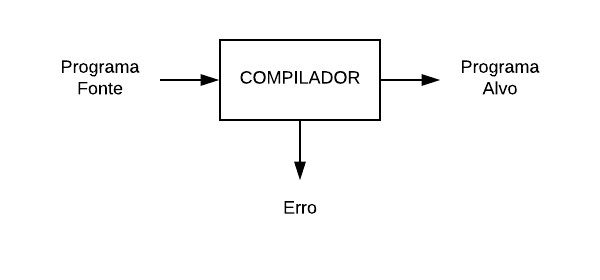
\includegraphics[width=250pt, height=100pt]{chapters/chapter1/figures/imagem1.png}
%%\centerline{\epsfig{/Chapters/chapter1/figures/cat.eps,width=.8\textheight,height=.4\textwidth}}
\caption[List of figure caption goes here]{Figure caption goes here.}
\end{figure}

\subsection{Programa fonte:} 
O programa fonte são arquivos escritos na linguagem de programação x, que será compilador em um compilador próprio para a linguagem x.\\

Todos os elementos  da linguagem presentes no código fonte são denominados “símbolos” que são elementos únicos e indivisíveis. Qualquer outro símbolo que não pertence a linguagem é considerado inválido. Estes símbolos fazem parte do alfabeto (Sigma) da linguagem, na \textbf{imagem 2}  temos o exemplo de um conjunto de símbolos (Alfabeto) da linguagem C.\\



IMAGEM 2\\ \\

O alfabeto $\Sigma$ é um conjunto de n símbolos de uma linguagem x. Este conjunto de símbolos possuí todos os elementos válidos da linguagem, ou seja, aquilo que a linguagem permite está presente neste conjunto.\\

Para reforçar os símbolos são elementos indivisíveis da linguagem, que fazem parte do conjunto denominado alfabeto, representado por $\Sigma$. Fazendo uma analogia, um símbolo da linguagem de programação é como uma letra de uma linguagem comum que falamos, que fazem parte do alfabeto.\\

Na implementação do compilador, os símbolos da linguagem são estruturas que possuem uma série de informações como: lexema, token, classe, endereço, padrão de formação e descrição.\\

IMAGEM 3\\ \\

Nesta sessão serão definidos os lexemas, tokens, padrão de formação e descrição. As classes e os endereços serão abordados nos CAPÍTULOS 7 E 8. \\

\subsubsection{Token}
Um token é um elemento do alfabeto $\Sigma$. Pode-se dizer que um token é um valor correspondente ao símbolo pertencente ao alfabeto. Representa uma unidade léxica. \\

IMAGEM 4\\ \\

\subsubsection{Lexema}
Um lexema é definido com as formas que um token pode ser escrito na linguagem. Tome o identificador como exemplo (id). O token do símbolo é id, porém o id pode ser escrito (nomeado) de várias formas diferentes. Estas formas são considerados os lexemas válidos para o token id. Um outro exemplo é o token constante, que pode ser representado por números na faixa de $-\infty$ á $+\infty$. Estas representações são os lexemas do token constante.\\

Dentre os símbolos do alfabeto o único que não é utilizado é o espaço em branço, está presente no alfabeto da linguagem mas não possui importância para a análise do compilador, sendo descartado nas primeiras fases do compilador. Pode-se considerar o espaço em branco apenas como um delimitador léxico.\\

IMAGEM 5\\ \\

\subsubsection{Padrão de formação de lexema}
É uma expressão regular que define a formação dos  lexemas de um token.\\

Exemplos na linguagem Pascal:\\

\begin{table}[!h]%1
%\noautomaticrules
\tabletitle{Now we are engaged $(a_g^a)$ $\big(a_g^a\big)$ in a great civil war, testing whether that
nation, or any nation so conceived.}%
\begin{tabular}{|c|c|c|}

\textbf{Token} & \textbf{Lexema} & \textbf{Padrão de formação} \\
\hline
constante & 0,-2,20,... & (-digito+ $\cup$ digito+)   \\
\hline
\textless & \textless & \textless\\
\hline
if   & If,IF,if,iF & (i $\cup$ I)(f $\cup$ F)\\
\hline
constante & "a", "String", "cadeia de caracteres" & "(Símbolos de $\Sigma$)"\\
\hline
while & While,WHILE,while & (W $\cup$ w)(h $\cup$ H)(i $\cup$ I)(l $\cup$ L)(e $\cup$ E)\\
\end{tabular}
\end{table}


\subsubsection{Descrição do símbolo} 
A descrição de símbolos é uma rotulação feita para identificar os símbolos em uma linguagem de programação. Na implementação do compilador esta informação não é utilizada, porém ela é de extrema importância para a separação e identificação dos símbolos da linguagem.\\

Estes rótulos são:

\begin{itemize}
\item Identificadores
\item Constantes numéricas
\item Constantes literais
\item Palavras Reservadas
\item Operador relacional
\end{itemize}

Exemplos:\\

\begin{table}[!h]%1
%\noautomaticrules
\tabletitle{Now we are engaged $(a_g^a)$ $\big(a_g^a\big)$ in a great civil war, testing whether that
nation, or any nation so conceived.}%
\begin{tabular}{|c|c|c|c|}

\textbf{Token} & \textbf{Lexema} & \textbf{Padrão de formação} & \textbf{Descrição} \\
\hline
constante & 0,-2,20,... & (-digito+ $\cup$ digito+) & Constante numérica \\
\hline
constante & "Cadeia de caracteres", ... & ("Símbolos de $\Sigma$")* & Constante literal\\
\hline
for & For, for, FOR, … & (f $\cup$ F)(o $\cup$ O)(r $\cup$ R) & Palavra reservada\\
\hline
identificador & a,ab,n,x, … & ($_ \cup$ d)($_ \cup$ d $\cup$ l)* & Identificador\\
\hline
if & if,If,IF & (i $\cup$ I)(f $\cup$ F) & Palavra reservada\\
\end{tabular}
\end{table}

\subsection{Programa alvo}
É um programa gerado pelo compilador, correspondente ao programa passado na entrada como mostra a \textbf{Figura 1}. Pode-se dizer que em quase todos os compiladores que o programa alvo é um programa Assembly de uma máquina específica.\\

IMAGEM 5\\

\section{Estrutura}

O compilador é dividivo em duas partes: A análise e a síntese.

\begin{figure}
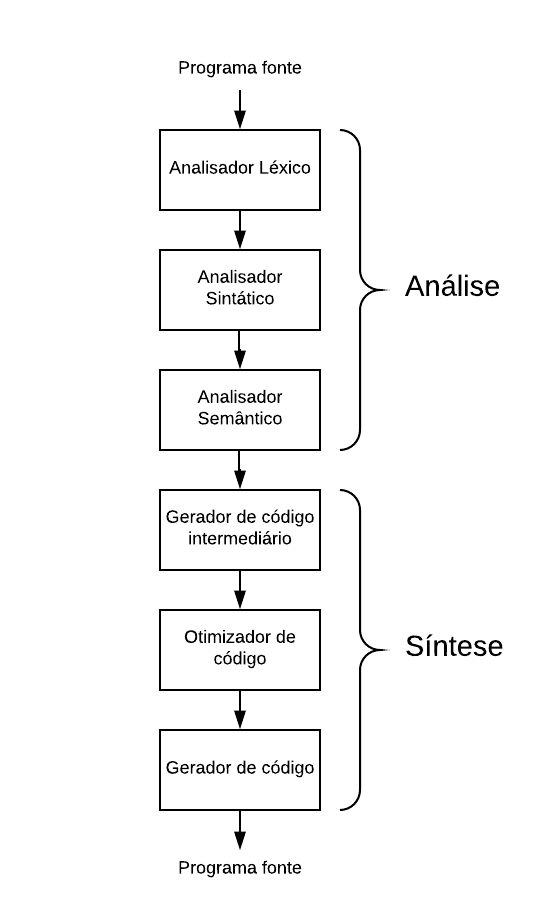
\includegraphics[width=337pt, height=320pt]{chapters/chapter1/figures/imagem6.png}
%%\centerline{\epsfig{/Chapters/chapter1/figures/cat.eps,width=.8\textheight,height=.4\textwidth}}
\caption[List of figure caption goes here]{Figure caption goes here.}
\end{figure}

\subsection{Análise}
É a parte que o compilador recebe o programa fonte e faz uma série de análises léxicas, sintáticas, e semânticas. É através da análise que caso o código fonte tenha erro o mesmo é gerado e tratado. É uma etapa que certifica que o arquivo fonte recebido na entrada está pronto para ser “tranformado” em código alvo.\\

A etapa de análise é dividida em 3: Analisador Léxico, Analisador Sintático, Analisador Semântico. \\

\subsubsection{Analisador Léxico}
Responsável por percorrer o código fonte realizando a identificação dos lexemas (ação semântica) e o atribuindo a um símbolo com seu token correspondente. É através do analisador léxico que comentários, espaços em branco são descartados. \\

IMAGEM 7\\

Fazendo uma alusão, podemos dizer que o processo do analisador léxico é como o processo de verificação de palavras em um texto, frase, poema, etc …\\

Vemos o exemplo abaixo, utilizando a linguagem de programação C e a língua portuguesa.


IMAGEM 7 E 8\\

\subsubsection{Analisador Sintático} 
É responsável por agrupar os tokens dos símbolos em estruturas hierárquicas. \\ 

Esta estrutura hierárquica denominado árvore de parse é fruto da derivação de uma gramática livre de contexto. Este processo de agrupamento tem a função de realizar a análise gramatical que é simplesmente conferir o que foi escrito no programa fonte com o que está na gramática da linguagem. \\

Fazendo alusão podemos dizer que o agrupamento de tokens na análise sintática é um agrupamento de palavras na linguagem falada. Não é possível verificar a coerência gramatical com apenas uma palavra. É necessário agrupar os elementos para que esta analise seja feita. \\

Tome parte de uma gramática livre de contexto GLC abaixo e parte da gramática da língua portuguesa. \\

\begin{center}
Linguagem C
\end{center}

G:\\ \\
\textbf{S} → int \textbf{Atribuicao} $|$ char \textbf{Atribuicao} $|$ byte \textbf{Atribuicao}\\
\textbf{Atribuicao} → id = \textbf{Valores};\\
\textbf{Valores} → const $|$ id \\ \\ \\

\begin{center}
Língua Portuguesa
\end{center}

G:\\ \\
\textbf{Oracao} → \textbf{Sujeito} \textbf{Predicado} \\
\textbf{Sujeito} → artigo substantivo \\
\textbf{Predicado} → \textbf{VerboLigativo} \textbf{PredicativoSujeito} \\
\textbf{VerboLigativo} → verbo \\
\textbf{PredicativoSujeito} → adjetivo

%\include{chapters/chapter2/ch2}

\part{Climate Risks in Public Health and Epidemiology}

\part{Socio-economic Impacts of Climate Adaptation and Resilience}



\bibliographystyle{plain}
\bibliography{bibtex_example}

\printindex

\end{document}
